\def\year{2018}\relax
%File: formatting-instruction.tex
\documentclass[letterpaper]{article} %DO NOT CHANGE THIS
\usepackage{aaai18}  %Required
\usepackage{times}  %Required
\usepackage{helvet}  %Required
\usepackage{courier}  %Required
\usepackage{url}  %Required
\usepackage{graphicx}  %Required
\frenchspacing  %Required
\setlength{\pdfpagewidth}{8.5in}  %Required
\setlength{\pdfpageheight}{11in}  %Required
%PDF Info Is Required:
  \pdfinfo{
/Title (Real Time Artificial Intelligence For Snake)
/Author (Ethan Larkham)}
\setcounter{secnumdepth}{0}
 \begin{document}
% The file aaai.sty is the style file for AAAI Press
% proceedings, working notes, and technical reports.
%
\title{Real Time Artificial Intelligence For Snake}
\author{Ethan Larkham\\
Department of Computer Science\\
University of New Hampshire\\
Durham, NH 03824 USA \\
ethanlarkham@protonmail.com\\
}
\maketitle
\begin{abstract}
  Snake when played in real-time can be a challenging puzzle to solve for a human, it's randomness leaves little room for flexibility and its speed leaves little room for thinking. This paper explores how well a computer would perform in this environment, given the same constraints and headaches that a human would experience. Three algorithms in total were implemented, while none of them were able to perfectly solve the problem, each perform fairly well depending on the parameters of their given environment. First a modified A* with contingency planning for when a path can't be found, next a Greedy Real-Time A* search and lastly a Hamilton Cycle generator. For both A* algorithms two heuristic functions were used, first is simply the Manhattan distance between the snake's head and the apple, second is a more complicated combination of heuristics that tries to stay away from the game's boundaries, keep close to the snake's tail and finally of course, find the apple.
\end{abstract}

\section{Introduction}
Snake is an old two dimensional arcade game where the player must control a "snake" and get it to consume the apple that is visible on screen. When the snake reaches the apple its body length increases by one and a new apple is randomly spawned somewhere else. If at any point in the game the snake touches itself or any of the four grid boundaries, the game ends and the player has lost. As the snake eats more apples, the size of its body increases and the game get progressively  more challenging to continue. If the player is able to increase the snake's size to the point that it is equal to the area of the grid that contains it, they will win the game.

In order to fully replicate the constraints and headaches a human might experience while trying to solve snake, I made my algorithms access to game logic completely asynchronous. Using the builtin features of my language of choice for this assignment: Golang, I have separated each algorithms computations onto it's own dedicated thread. It receives the same state updates that the game's renderer requires to draw it and is expected to respond to each of these state updates with an action designating the snakes movement. If the main thread attempts to receive the algorithm's action before the algorithm has delivered it, a timeout will occur and the main thread will fallback to whatever action was used in the prior iteration.

\begin{figure}[h]
  \centering
  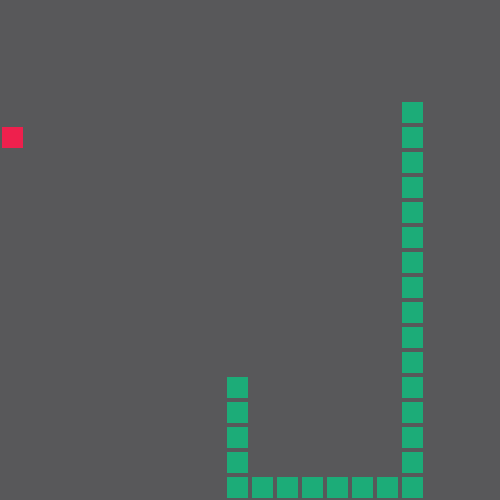
\includegraphics[height=5cm]{../screenshots/game}
  \caption{Gameplay}
  \label{fig:gameplay}
\end{figure}

\section{Modified A* With Contingency Planning}
My first approach to the problem was using a basic A* algorithm with, the idea was that the path would only be calculated when the snake reached an apple. The discovered path would be saved by the A* thread and the actions required to replicate it would be sent off to the main thread until the next apple was reached. If the calculation takes to long then a timeout would just occur and the A* thread would just have to try again on the next tick, of course this leaves the snake liable to collision, so ideally timeouts are to be avoided.

One major downside to snake's volatile game state is it prevents reuse of G or F scores from prior path calculations, pretty much any kind of real-time learning just hasn't been practical. Another common issue that arises with this volatility, is as the snake's body increases, there will be periods where there is simply no paths to the apple. During these periods a human player would have to perform actions that attempt to compress the snake's body mass into something that isn't a glob of spaghetti and opening the necessary path to get to the apple. In an effort to capture this strategy, my tweaked version of A* will fallback to a more greedy nature when attempts to find a path fail. These counter measures work similarly to my Greedy RTA* algorithm and simply calculates the weights of the children adjacent to the head, allowing for almost a computer's intuition to be used in cases where there are no other options.

\section{Greedy Real-Time A*}
 My Greedy Real-Time A* algorithm is a very chiseled down version of a more traditional RTA* implementation. Unfortunately since Snake's volatile environment negates most learning techniques, much of RTA*'s strengths were left out of my reach. My version works by doing what would be best described as a single depth A* search, since it's computationally very cheap, the next action is calculated every tick rather than only when an apple is reached like with my other A* algorithm. The primary strength of this algorithm's cheap and greedy nature is that unlike A*, it can perform reasonably well in nearly any sized environment and will in practice never timeout.

 Since the maximum amount of children the snake's head can have is three (it can't move backwards), each child effectively provides a weight in the form of an f-score to the three corresponding directions the snake can move in, whichever has the best score is the one chosen as the action to be shipped off to the main thread. I believe this algorithm can work very well as something to integrate into other algorithms, such as what I've done with my other A* algorithm. Once the snake reaches a certain size threshold, this algorithm will nearly always fail since it simply can't take into account the additional complexity, however in cases where a clear path can't be found, this is an excellent temporary alternative.

\section{Hamilton Cycle Generation}
Of my three algorithms this one is the only one that has been actually able to beat the game. It works via the simple trick of calculating the Hamiltonian path of the game grid. This in effect, creates a cyclical path that visits each vertex exactly once. So instead of bothering to find a path to the apple the snake just visits every possible location the apple could be in. The beauty of this method is that by following this path you are able to guarantee that the snake will never collide with itself until the game is won.

To my surprise, it is actually pretty computationally cheap to calculate one of these cycles. I had originally anticipated having to make an additional thread to calculate the cycle while the primary one just tells the snake to spin in circles, but not even that was necessary. The downsides to this approach are that my implementation doesn't work with grids with an odd number of tiles, and that while pretty neat, is kind of boring. Calculating Hamilton cycles for grids with an odd number of tiles is definitely possible but was not something I was able to accomplish in time. There is however the possibility that alternative approaches that could work with an odd number of tiles would be more computationally expensive.


\section{Evaluation}
For my evaluation I ran each of my algorithms 20 times each with a delay of 10ms and a 20x20 grid. Performance is primarily measured by comparing the ratio between the snakes body length and the area of the grid, however other metrics were recorded such as average amount of actions required to reach the apple. My A* algorithm was measured twice with a simple Manhattan distance heuristic and a more advanced one that tries to stay close to its tail.

 Figure 1 shows the average board ratios for each method, in Hamilton with it's 100 percent success rate demonstrates the highest which wasn't much of a surprise. The downsides to Hamilton's success can be seen in Figure 2 which shows it also has the highest actions per apple, in the case of real-time pathing minimizing actions per apple was never one of my intentions however this could pose a problem to others who may desire the snake to get the apples fast, in contrast to my desire to make its general decisions fast.

\begin{figure}[h]
  \centering
  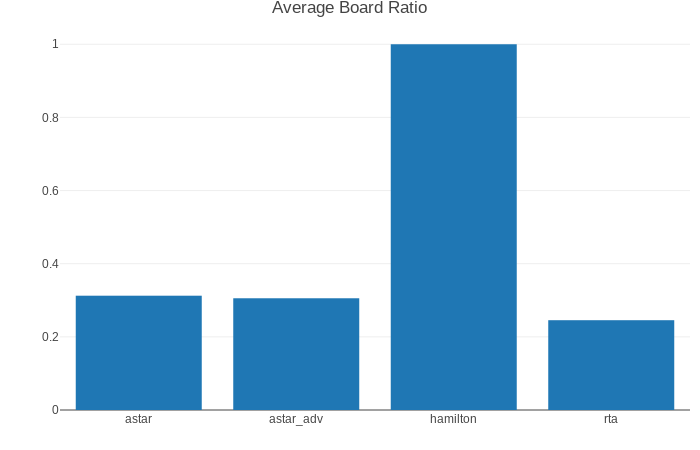
\includegraphics[height=5cm]{../graphs/avg_board_ratio}
  \caption{Average Board Ratio}
  \label{fig:board_ratio}
\end{figure}

\begin{figure}[h]
  \centering
  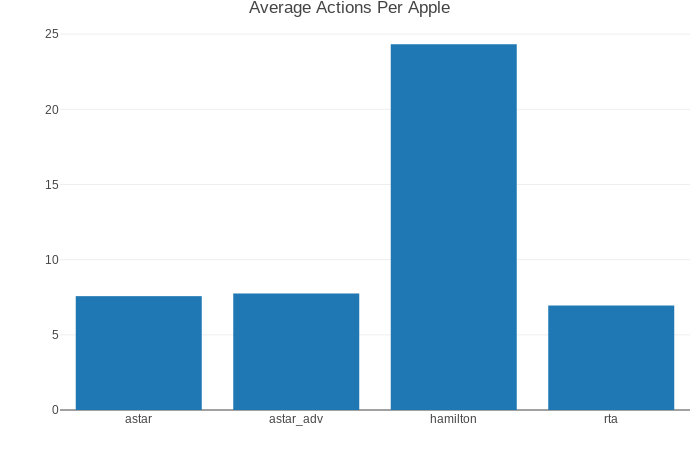
\includegraphics[height=5cm]{../graphs/avg_actions_per_apple}
  \caption{Average Actions Per Apple}
  \label{fig:actions_per_apple}
\end{figure}


\section{Conclusion}
While the early game is fairly simple, actually pushing your way through the late game and beating the game is actually very challenging when given a time-limit. While certain strategies can be manually programmed in, nothing I have found beyond Hamilton cycles can actually beat the game, and even with Hamilton cycles, it's not quite done at the same speeds or efficiencies that a skilled human player would be capable of. My suggestion to anyone in the future that attempts something similar to this would be to try using some kind of machine learning algorithm, I think there is a lot of nuance to the game that is just not easily understood by humans that machine learning algorithms could probably find. Overall I think for my A* algorithms the more advanced heuristics as well as the contingency plans definitely had some impact, so if machine learning was out of the question, expanding on those aspects would be a great place to expand upon.

\cite{*}
\bibliography{ai_final_report}
\bibliographystyle{aaai}
\end{document}
